\documentclass[10pt]{article}
\usepackage[margin=0.9in]{geometry}
\usepackage[T1]{fontenc}
\usepackage{lmodern}
\usepackage{amsmath,amssymb}
\usepackage{graphicx}
\usepackage{booktabs}
\usepackage{xcolor}
\usepackage[numbers,sort&compress]{natbib}
\usepackage[colorlinks=true,linkcolor=blue!50!black,citecolor=blue!50!black,urlcolor=blue!50!black]{hyperref}
\usepackage{tikz}
\usetikzlibrary{positioning,arrows.meta,fit,calc}
\usepackage{enumitem}
\setlist{nosep,leftmargin=*}
\usepackage{titlesec}
\titlespacing*{\section}{0pt}{6pt}{3pt}
\titlespacing*{\subsection}{0pt}{4pt}{2pt}
\setlength{\parskip}{2pt}

\newcommand{\R}{R}
\renewcommand{\Pr}{P}

\title{\vspace{-1.5em}\textbf{Useful but Not Revealing:}\\
Prompt-Conditioned, Privacy-Aware Visual Token Pruning for Vision-Language Models\\[2pt]
\large Project Proposal}
\author{Ahmed Abdelnaby}
\date{}

\begin{document}
\maketitle
\vspace{-2.5em}

\begin{abstract}
\noindent
Vision-language models (VLMs) turn every image into hundreds of visual tokens and feed all of them to a large language model (LLM),
including tokens showing faces, names, license plates or ID documents that are irrelevant to the user's question.
Existing visual-token pruning methods discard tokens only to save computation and ask \emph{which tokens are unnecessary}.
We propose to ask \emph{which tokens are useful \textbf{and} safe}. For each visual token $i$ we estimate a
question-dependent task relevance $\R_i$ and a question-independent privacy risk $\Pr_i$, and keep the top-$K$ tokens
of $S_i=\R_i-\lambda \Pr_i$. We build this on a frozen LLaVA-1.5-7B, obtain token-level privacy ground truth from the
pixel-level VISPR-redactions annotations, and measure the resulting privacy--utility--efficiency trade-off with geometric,
behavioural and representational privacy metrics.
\end{abstract}

\section{Problem and Motivation}
\textbf{Problem.} Given an image $I$ and a question $q$, a VLM such as LLaVA-1.5~\cite{liu2024llava15} encodes $I$ into
$N=576$ visual tokens $z_1,\dots,z_N$ (a $24{\times}24$ grid of CLIP~\cite{radford2021clip} patches) and conditions the LLM on all of them.
We study the question: \emph{can we choose a budget of $K<N$ tokens that preserves the information needed to answer $q$ while
withholding privacy-sensitive content?}

\textbf{Why it matters.} (i) Personal images routinely contain private attributes such as faces, names, addresses and documents~\cite{orekondy2017vispr};
VLMs can infer such attributes at scale~\cite{tomekce2024private}. (ii) Deployments increasingly split inference between a device and a cloud LLM.
Every visual token sent to the server is a potential leak, and pruning is a natural place to enforce data minimisation.
(iii) Token pruning is already needed for efficiency~\cite{chen2024fastv,zhang2025sparsevlm,zhang2025vispruner,alvar2025divprune}.
Making it privacy-aware adds protection at no extra inference cost, and the pruned model is \emph{faster} than the original.
(iv) Blurring or masking pixels is known to be defeated by learned models~\cite{mcpherson2016defeating}.
Removing tokens from the model's input is a different, representation-level form of redaction whose effectiveness is untested.

\textbf{Hypothesis.} The tokens that are important for a downstream question are largely \emph{not} the tokens that carry private
information. Modelling both explicitly therefore retains task utility while suppressing private content, improving on
relevance-only pruning at the same token budget.

\section{Relation to Prior Work}
\textbf{Visual-token reduction.} FastV~\cite{chen2024fastv} drops image tokens that receive little attention after layer 2.
SparseVLM~\cite{zhang2025sparsevlm} uses text-guided scoring, and VisPruner~\cite{zhang2025vispruner} argues that text--visual attention
is an unreliable signal and uses visual cues instead. DivPrune~\cite{alvar2025divprune} maximises the diversity of the kept tokens,
and ToMe~\cite{bolya2023tome} merges similar tokens inside the ViT. All of these optimise \emph{efficiency--utility} only.
Our relevance term $\R_i$ is interchangeable with any of their scores; our contribution is the privacy term $\Pr_i$ and the
evaluation of what pruning does to privacy.
\textbf{Visual privacy.} VISPR~\cite{orekondy2017vispr} defines 67 image privacy attributes. The redaction extension~\cite{orekondy2018redactions}
adds pixel-level polygons for about 24 localisable attributes and shows that redacting those regions gives privacy while retaining utility.
Those methods redact \emph{pixels} for human viewers; we redact \emph{tokens} for a model and make the redaction depend on the question.

\section{Technical Plan}
\begin{figure}[t]
\centering
\resizebox{\linewidth}{!}{%
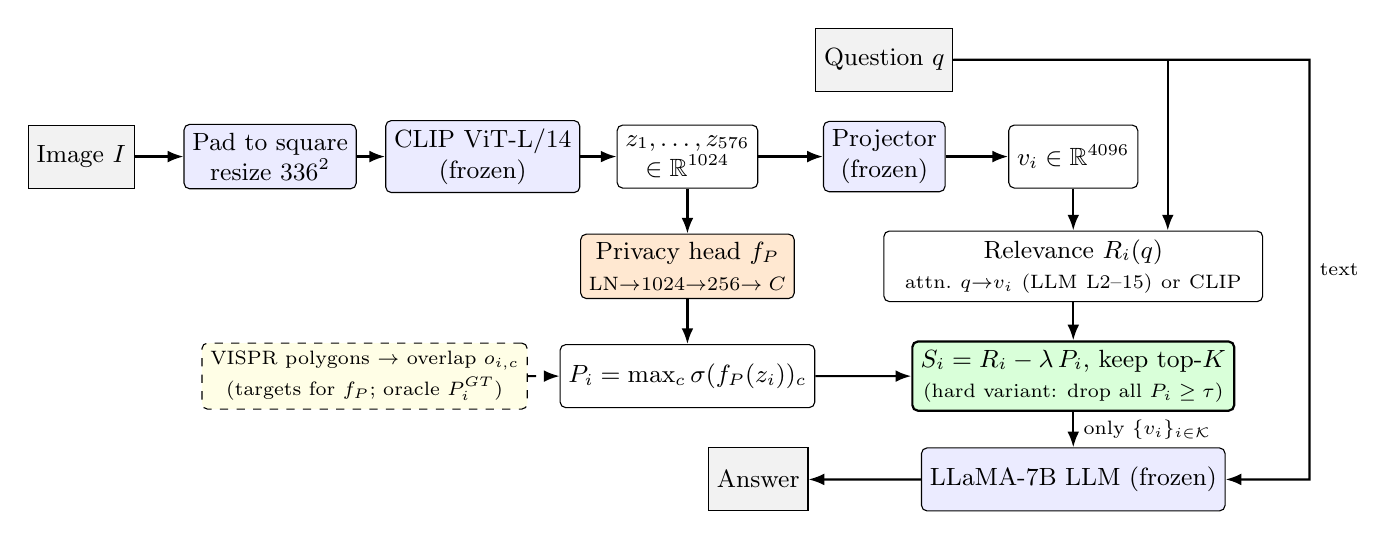
\begin{tikzpicture}[yscale=0.82,
  node distance=5mm and 7mm,
  box/.style={draw,rounded corners=2pt,align=center,font=\small,minimum height=8mm,inner sep=3pt},
  frozen/.style={box,fill=blue!8},
  train/.style={box,fill=orange!18},
  ours/.style={box,fill=green!15,thick},
  io/.style={box,fill=gray!10,sharp corners},
  arr/.style={-{Latex[length=2mm]},thick}]
% row 1: vision path
\node[io]     (img)  at (0,0)    {Image $I$};
\node[frozen] (pad)  at (2.4,0)  {Pad to square\\resize $336^2$};
\node[frozen] (vit)  at (5.1,0)  {CLIP ViT-L/14\\(frozen)};
\node[box]    (z)    at (7.7,0)  {$z_1,\dots,z_{576}$\\$\in\mathbb{R}^{1024}$};
\node[frozen] (proj) at (10.2,0) {Projector\\(frozen)};
\node[box]    (v)    at (12.6,0) {$v_i\in\mathbb{R}^{4096}$};
\node[io]     (q)    at (10.2,1.5) {Question $q$};
% row 2: scoring
\node[train]  (ph)   at (7.7,-1.7) {Privacy head $f_P$\\\scriptsize LN$\to$1024$\to$256$\to C$};
\node[box,text width=46mm] (R) at (12.6,-1.7) {Relevance $\R_i(q)$\\\scriptsize attn.\ $q{\to}v_i$ (LLM L2--15) or CLIP};
% row 3: selection and answer
\node[box,dashed,fill=yellow!10] (gt) at (3.6,-3.4) {\scriptsize VISPR polygons $\to$ overlap $o_{i,c}$\\\scriptsize (targets for $f_P$; oracle $\Pr^{GT}_i$)};
\node[box]    (P)    at (7.7,-3.4) {$\Pr_i=\max_c \sigma(f_P(z_i))_c$};
\node[ours]   (S)    at (12.6,-3.4) {$S_i=\R_i-\lambda\,\Pr_i$, keep top-$K$\\\scriptsize (hard variant: drop all $\Pr_i\ge\tau$)};
\node[frozen] (llm)  at (12.6,-5.0) {LLaMA-7B LLM (frozen)};
\node[io]     (ans)  at (8.6,-5.0) {Answer};
\draw[arr] (img)--(pad); \draw[arr] (pad)--(vit); \draw[arr] (vit)--(z); \draw[arr] (z)--(proj); \draw[arr] (proj)--(v);
\draw[arr] (z)--(ph); \draw[arr] (ph)--(P); \draw[arr] (v)--(R); \draw[arr] (R)--(S);
\draw[arr] (q.east)-|([xshift=12mm]R.north);
\draw[arr] (q.east)-|(15.6,-5.0) node[pos=0.75,right,font=\scriptsize]{text}--(llm.east);
\draw[arr] (P)--(S);
\draw[arr] (S)--(llm) node[midway,right,font=\scriptsize]{only $\{v_i\}_{i\in\mathcal K}$};
\draw[arr] (llm)--(ans);
\draw[arr,dashed] (gt)--(P);
\end{tikzpicture}}
\caption{Proposed pipeline. Blue: frozen LLaVA-1.5 components. Orange: the only trained module (${\approx}0.27$M parameters).
Green: privacy-aware selection. The LLM receives only the $K$ selected visual tokens, in their original raster order.}
\label{fig:arch}
\end{figure}

\subsection{Setting and model}
We use LLaVA-1.5-7B~\cite{liu2024llava15} with all weights frozen. The image is padded to a square (as in LLaVA-1.5) and resized to $336^2$;
CLIP ViT-L/14-336 produces $576$ patch features $z_i$ (layer $-2$), which a 2-layer MLP projects to LLM embeddings $v_i$.
To prune, we build the LLM input ourselves, \texttt{[text before image | $v_i$ for $i\in\mathcal K$ | question]}, and call
generation with these embeddings, so dropped tokens are never seen by the LLM.
With $\mathcal K$ = all tokens, this reproduces the reference Hugging Face implementation exactly (max logit difference $0.0$ in our tests).

\subsection{Privacy risk $\Pr_i$ (question-independent)}
\textbf{Token-level ground truth.} VISPR-redactions~\cite{orekondy2018redactions} provides polygons for 28 privacy attributes
(face, person, nudity, name, address, phone, e-mail, license plate, passport, credit card, signature, \dots).
We apply exactly the same pad-and-resize to the polygons, rasterise them at $4\times$ resolution, and average-pool to the $24{\times}24$ grid:
\begin{equation}
o_{i,c}=\frac{|A_i\cap M_c|}{|A_i|},\qquad \Pr^{GT}_i=\frac{|A_i\cap \bigcup_c M_c|}{|A_i|}\in[0,1],
\end{equation}
where $A_i$ is the $14{\times}14$ patch of token $i$ and $M_c$ the mask of class $c$ (Fig.~\ref{fig:masks}).
\textbf{Learned risk.} A small head $f_P$ (LayerNorm$\to$Linear(1024,256)$\to$GELU$\to$Linear(256,$C$)) maps each frozen $z_i$ to
multi-label probabilities $p_{i,c}=\sigma(f_P(z_i))_c$. We use sigmoids rather than a softmax because attributes overlap (face $\subset$ person).
It is trained on the \emph{soft} targets $o_{i,c}$ with class-weighted BCE,
$\mathcal L=-\sum_{i,c}\big[w_c^{+}o_{i,c}\log p_{i,c}+(1-o_{i,c})\log(1-p_{i,c})\big]$, with $w_c^{+}=\min(\text{neg}_c/\text{pos}_c,100)$, so that
rare classes (passport, credit card) are not swamped by face/person. At inference $\Pr_i=\max_c p_{i,c}$, with equal class weights.
Severity-weighted variants are an ablation, because hand-picked severities are hard to justify.

\begin{figure}[t]
\centering
\includegraphics[width=0.9\linewidth]{figs/mask_check.png}
\vspace{-1.5em}
\caption{Token-level privacy ground truth $\Pr^{GT}_i$ (red) on random VISPR-redactions test images, after LLaVA's pad-and-resize.
Titles list the annotated attributes. 28.7\% of test tokens have $\Pr^{GT}_i>0.25$, dominated by \emph{person} and \emph{face}.}
\label{fig:masks}
\vspace{-0.5em}
\end{figure}

\subsection{Task relevance $\R_i$ (question-dependent)}
\textbf{R1: attention (main).} We run the first 16 LLM layers on the full sequence (a FastV-style cheap pass) and average the attention
from the question tokens $Q$ to visual token $i$ over layers $\mathcal L=\{2,\dots,15\}$ and all heads $H$:
$\tilde \R_i=\frac{1}{|\mathcal L||H||Q|}\sum_{l,h,t\in Q}A^{l,h}_{t,i}$.
\textbf{R2: CLIP text--patch similarity.} $\tilde\R_i=\cos(W_v \hat z_i, e_q)$ uses CLIP's own text encoder and MaskCLIP value features~\cite{zhou2022maskclip}.
It needs no LLM pass, so it remains valid when the LLM is untrusted (see below).
\textbf{R3: leave-block-out (oracle).} $\tilde\R_i=\max\!\big(0,\log p(y\,|\,\text{all})-\log p(y\,|\,\text{all}\setminus b(i))\big)$
for $2{\times}2$ blocks $b$ and the full-image answer $y$. It needs 144 teacher-forced passes, so it serves only as an upper bound.
\textbf{Normalisation.} LLaVA exhibits high-norm ``attention-sink'' tokens~\cite{darcet2024registers}, which make min--max scaling squash most $\R_i$ to ${\approx}0$,
so the effective strength of $\lambda$ would vary per image. We therefore rank-normalise, $\R_i=\mathrm{rank}(\tilde\R_i)/(N-1)$, and keep min--max as an ablation.

\subsection{Privacy-aware selection}
With $x_i\in\{0,1\}$ indicating a kept token, we solve
\begin{equation}
\max_{x}\ \sum_i x_i\R_i-\lambda\sum_i x_i\Pr_i\quad\text{s.t.}\quad \sum_i x_i=K,
\end{equation}
whose exact solution is to keep the top-$K$ tokens of $S_i=\R_i-\lambda\Pr_i$ (\emph{soft}). $\lambda$ traces the privacy--utility curve,
and $\lambda=0$ recovers relevance-only pruning. A \emph{hard} variant never admits $\Pr_i\ge\tau$.
It matters because $\R_i$ depends on the question: an adversarial question (``What is the person's name?'') pulls relevance onto exactly the private tokens.
The soft score can then be outweighed by high relevance, whereas the hard gate cannot.

\textbf{Threat models.} (a) \emph{Output leakage}: the VLM is trusted, and the answer must not reveal private content.
(b) \emph{Split inference}: only the kept tokens leave the device. Under (b), attention-based $\R$ is invalid because computing it exposes all tokens,
so R2 is the deployable variant and R1 an upper reference.

\section{Experimental Plan}
\textbf{Data.} VISPR-redactions~\cite{orekondy2018redactions}: 3,873 / 1,611 / 2,989 train/val/test images with polygons (train/val for $f_P$, test for evaluation).
GQA testdev-balanced~\cite{hudson2019gqa} provides labelled utility (no privacy masks, so it uses the learned $\Pr$).
HR-VISPR (human-centred privacy labels) will serve as a cross-dataset generalisation test for $f_P$.

\textbf{Tasks per VISPR test image.} (1) Privacy-neutral utility questions (scene, indoor/outdoor, colour), scored by agreement with the full-token answer.
(2) \emph{Privacy probes}: the official VISPR yes/no question for each present attribute (e.g.\ ``Is someone's face visible?'').
These are asked \emph{adversarially} (tokens selected with the probe as $q$) and \emph{benignly} (tokens selected for a neutral question).
(3) Probes for absent attributes, to control for a model that simply answers ``yes''.

\textbf{Metrics.} \emph{Geometric privacy}: private-token retention $\mathrm{PTR}=\sum_i x_i\Pr^{GT}_i/\sum_i\Pr^{GT}_i$ ($\downarrow$).
\emph{Behavioural privacy}: probe leakage, i.e.\ the ``yes'' rate on present attributes ($\downarrow$).
\emph{Representational privacy}: mAP of a linear attribute probe trained on mean-pooled kept tokens ($\downarrow$). This tests whether private information
survives in the \emph{remaining} tokens, since ViT self-attention mixes information across patches.
\emph{Utility}: agreement with the full-token answer and GQA accuracy ($\uparrow$). \emph{Efficiency}: kept tokens, prefill latency ($\downarrow$).

\textbf{Baselines and grid.} Full (576 tokens); random; relevance-only ($\lambda{=}0$); privacy-only ($-\Pr$); ours soft
$\lambda\in\{0.1,0.25,0.5,1,2\}$ and hard $\tau\in\{0.5,0.8\}$; budgets $K/N\in\{75,50,25,10\}\%$.
Existing pruners (FastV, VisPruner, DivPrune) plug in as alternative $\R$.

\begin{table}[t]
\centering\small
\begin{tabular}{@{}llll@{}}
\toprule
Exp. & $\R$ & $\Pr$ & Question answered \\
\midrule
E1 & attention / CLIP & oracle $\Pr^{GT}$ & Does privacy-aware selection work at all? \\
E2 & leave-block-out & oracle $\Pr^{GT}$ & Best achievable trade-off (upper bound) \\
E3 & attention & learned $f_P$ & Cost of an imperfect privacy estimate \\
E4 & CLIP & learned $f_P$ & Deployable split-inference system \\
E5 & attention & learned (VISPR$\to$HR-VISPR) & Cross-dataset generalisation \\
\bottomrule
\end{tabular}
\caption{Experiments. Oracle-$\Pr$ experiments come first: if they show no gain, the learned head is not worth building.}
\label{tab:exp}
\vspace{-1em}
\end{table}

\textbf{Implementation status and first results.} The full pipeline is implemented and has been run end to end: token labels, features,
$f_P$, and evaluation on 200 VISPR test images (2,062 tasks) plus 300 GQA questions. The learned head reaches a token-level AP of 0.87 for ``private vs.\ not''
on the test set (class-mean AP 0.48 over 28 attributes). Table~\ref{tab:first} reports E1/E3 at $K{=}288$ (50\%).
Three observations shape the rest of the project.
(i) Relevance-only pruning keeps \emph{more} private tokens than random pruning (PTR 0.66 vs.\ 0.49), because attention is drawn to people and text.
(ii) With learned $\Pr$ and $\lambda{=}1$, PTR drops to 0.20 with \emph{no} loss of GQA accuracy.
(iii) Removing tokens does not remove all information. Adversarial leakage and attribute recoverability fall far less than PTR, which is the token-mixing effect.
Interestingly, the learned $\Pr$ lowers leakage \emph{more} than the oracle masks at the same $\lambda$ (0.30 vs.\ 0.49 at $\lambda{=}2$), plausibly because
it also flags contextual tokens that carry private information. The hard gate trades about 4 GQA points for near-zero leakage.

\begin{table}[h]
\centering\small
\setlength{\tabcolsep}{4.5pt}
\begin{tabular}{@{}lcccccc@{}}
\toprule
Method ($K{=}288$, attention $\R$) & VISPR util.$\uparrow$ & GQA acc.$\uparrow$ & PTR$\downarrow$ & Adv.\ leak$\downarrow$ & Benign leak$\downarrow$ & Recover.\ mAP$\downarrow$ \\
\midrule
Full (576 tokens) & 1.00 & 0.600 & 1.00 & 0.79 & 0.79 & 0.81 \\
Random & 0.86 & 0.583 & 0.49 & 0.72 & 0.72 & 0.80 \\
Relevance only ($\lambda{=}0$) & 0.87 & 0.600 & 0.66 & 0.72 & 0.72 & 0.79 \\
Soft, oracle $\Pr^{GT}$, $\lambda{=}2$ & 0.86 & -- & 0.07 & 0.49 & 0.44 & 0.69 \\
Soft, learned $\Pr$, $\lambda{=}1$ & 0.87 & 0.600 & 0.20 & 0.54 & 0.47 & 0.71 \\
Soft, learned $\Pr$, $\lambda{=}2$ & 0.84 & 0.557 & 0.13 & 0.30 & 0.27 & 0.68 \\
Hard, learned $\Pr$, $\tau{=}0.5$ ($\bar K{=}239$) & 0.74 & 0.560 & 0.07 & 0.05 & 0.05 & 0.54 \\
\bottomrule
\end{tabular}
\caption{First results (200 VISPR test images, 300 GQA questions). Utility is agreement with the full-token answer. Leakage is the ``yes'' rate on present-attribute probes
(false-``yes'' rate on absent attributes: at most 0.08 for all rows). Oracle masks are unavailable for GQA.}
\label{tab:first}
\vspace{-1em}
\end{table}

\textbf{Timeline.} Done: pipeline, E1/E3, privacy head, recoverability. Wk 1: E2 (oracle relevance) and E4 (CLIP relevance, full analysis).
Wk 2: explain the learned-vs-oracle gap (dilated oracle masks) and add in-ViT pruning against token mixing. Wk 3: ablations ($\lambda$, $\tau$, normalisation,
severity weights, excluding \emph{person}). Wk 4: HR-VISPR generalisation and existing-pruner baselines. Wk 5--6: larger evaluation and the report.

\textbf{Risks and mitigations.} (i) \emph{Token mixing} may keep leakage high even at PTR${\approx}0$. Mitigation: prune inside the ViT (earlier layers) or mask its
attention to private patches; Table~\ref{tab:first} already shows the effect. (ii) \emph{Coarse masks} (e.g.\ \emph{person} covering whole scenes)
conflate privacy with utility. We report per-attribute results and an ablation excluding \emph{person}. (iii) \emph{Weak utility signal} from easy neutral questions,
addressed with GQA. (iv) \emph{Compute}: about 40\,s per image for the full grid on one RTX 4090. The grid is resumable and de-duplicates identical token sets.

{\footnotesize
\setlength{\bibsep}{1pt}
\bibliographystyle{abbrvnat}
\bibliography{refs}
}
\end{document}
